\documentclass{cours}
\usetikzlibrary{decorations.pathreplacing}
\renewcommand{\res}{\boxed}
\begin{document}
\setcounter{section}{0}
\chapter{Optique géométrique}
\section{sources de lumière}
\subsubsection{Définitions :}
\begin{description}
\item[Une source de lumière] est un objet qui émet de la lumière
\item[Une source primaire] est une source qui produit la lumière qu'elle émet
\item[Une source secondaire] est une source qui diffuse la lumière qu'elle reçoit
\end{description}

Une source lumineuse peut émettre plusieurs longueurs d'onde (couleurs) simultanément. Le \textbf{spectre} de la lumière correspond à l'intensité de l'ensemble des longueurs d'onde émises : $I(\lambda)$.

\begin{center}
\usetikzlibrary{decorations.pathmorphing}
  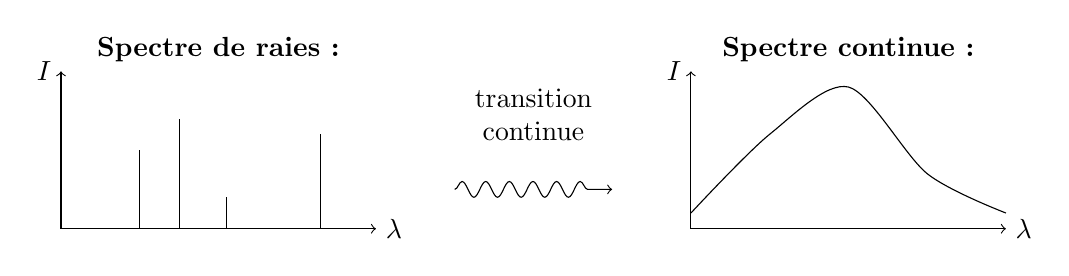
\begin{tikzpicture}
    %Spectre de raies
    \draw (2,2) node[above] {\textbf{Spectre de raies :}};
    \draw[->] (0,0) -- (4,0) node[right]{$\lambda$};
    \draw[->] (0,0) -- (0,2) node[left]{$I$};
    \draw (1,0) -- (1,1) (1.5,0) -- (1.5,1.4) (2.1,0) -- (2.1,0.4) (3.3,0)--(3.3,1.2) ;

   %Spectre continue
    \draw (10,2) node[above] {\textbf{Spectre continue :}};
    \draw[->] (8,0) -- (12,0) node[right]{$\lambda$};
    \draw[->] (8,0) -- (8,2) node[left]{$I$};
    \draw plot[smooth] coordinates {(8,0.2) (9,1.2) (10,1.8) (11,0.7) (12,0.2)};

   %Transition
    \draw (6,1) node[above,align=center] {transition\\ continue};
    \draw[->,decorate, decoration={snake,amplitude=1mm,segment length=3mm, post length=2mm}] (5,0.5) -- (7,0.5);
  \end{tikzpicture}
\end{center}

\textbf{Une source ponctuelle monochromatique} est une source idéale réduite à un point dont le spectre ne contient qu'une seule longueur d'onde. 

\textbf{Attention ! :} C'est un modèle, les raies d'une source réelle ont toujours une certaine largeur :
\begin{center}
  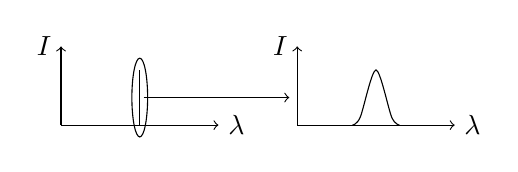
\begin{tikzpicture}
    \draw[->] (0,0) -- (2,0) node[right]{$\lambda$};
    \draw[->] (0,0) -- (0,1) node[left]{$I$};
    \draw (1,0) -- (1,0.7);
    \draw (1,0.35) ellipse (0.1 and 0.5);
    \draw[->] (1.05,0.35) -- (2.9,0.35);

    \draw[->] (3,0) -- (5,0) node[right]{$\lambda$};
    \draw[->] (3,0) -- (3,1) node[left]{$I$};
    \draw plot[smooth] coordinates{(3.7,0) (3.8,0.1) (4,0.7) (4.2,0.1) (4.3,0)};

  \end{tikzpicture}
\end{center}


\section{Indice d'un milieu}
Dans l'ensemble de se chapitre on étudiera des milieux \textbf{transparents}, \textbf{homogènes} et \textbf{isotropes}.
\begin{description}
\item[transparent : ] La lumière traverse le milieu sans que son intensité ne soit atténuée ; 
\item[homogène : ] les propriétés de propagation de la lumière sont les mêmes en tout point de l'espace ;
\item[isotrope :] les propriétés de propagation de la lumière sont les mêmes dans toutes les directions.  
\end{description}

Dans le vide, la lumière se propage à la vitesse $c=\SI{299792458}{m/s} \simeq \SI{3e8}{m/s}$. Dans un matériau transparent homogène et isotrope, elle se propage à $v=\frac{c}{n}$

$n$ est \textbf{l'indice de réfraction} du milieu.

\begin{center}
  \begin{tabular}{@{}lllll@{}}
    \toprule
    eau & air & diamant & verre \\
    1.33 & 1.0003 & 2.42 & 1.46 \\
    \bottomrule
  \end{tabular}
\end{center}
Lorsqu'une onde lumineuse passe du vide à un milieu, sa fréquence reste inchangée mais sa longueur d'onde change :
\begin{equation*}
\lambda_m = \frac{v}{f} = \frac{c}{nf} = \frac{\lambda}{n} \quad \text{donc} \quad \lambda_m=\frac{\lambda}{n}
\end{equation*}
\begin{itemize}
\item $\lambda_m$ : longueur d'onde dans le milieu
\item $\lambda$ : longueur d'onde dans le vide
\end{itemize}
\section{Approximation de l'optique géométrique}
\subsection{Observation}
Dans un milieu transparent, homogène, isotrope, la lumière se propage en ligne droite
\subsection{Modèle}
On symbolise le trajet de la lumière par un \textbf{rayon lumineux} d'épaisseur nulle représenté par une droite orientée. 

\begin{center}
\begin{tikzpicture}
\draw (0,0) node[circle,fill=black,inner sep=1pt](S){} node[above,black] {Source};
\draw[rayon, coul1] (S.east) -- (9,0) node[pos=0.5, above,black] {Rayon lumineux} ;
\draw (9,-1) -- (9,1) node[right] {\'Ecran};
\end{tikzpicture}
\end{center}
\textbf{Attention :} C'est un modèle, un rayon lumineux n'existe pas, la diffraction interdit d'isoler un rayon lumineux unique.
\begin{center}
  \begin{tikzpicture}
    \draw (0,0) rectangle (2,0.5) node[pos=0.5] {Laser};
    \draw[draw=none,fill=coul1,opacity=0.4] (2,0.1) rectangle (4,0.4);
    %Diaphragme
    \draw[thick] (4,-0.8) node[below]{Diaphragme} -- (4,0.2) (4,0.3) -- (4,1.05);
    \draw[->] (4.2,0.7) node[right] {$D$} --(4.2,0.4);
    \draw[->] (4.2,-0.2) --(4.2,0.1);
    %Ecran
    \draw (7,-1) node[right] {\'Ecran}-- (7,1.25);
    
    \draw[draw=none,fill=coul1,opacity=0.4] (4,0.3) -- (7,0.7) -- (7,-0.2) -- (4,0.2) -- cycle;

    \draw ([shift=(-10:1)]4,0.25) arc (-10:10:1) node[right] at (5,0.25) {$\theta=\dfrac{\lambda}{D}$} ;

  \end{tikzpicture}
  \captionof{figure}{Diffraction d'un faisceau lumineux par une ouverture.}
\end{center}
\section{Réflexion - réfraction}
\subsection{Réflexion}
  \usetikzlibrary{decorations.markings}
  \begin{center}
  \begin{tikzpicture}[decoration = {markings, mark=at position 0.5 with{\arrow{>}}}]
    %tikz optique
    \draw (0,0) -- (5,0) node[anchor=south west,align=center] {normale à \\la surface};
    \draw (4,-1) --(4,1);
    \foreach \y in {-1,-0.9,...,1.1} {
      \draw (4,\y) --++ (0.1,0.1);
    }
    \draw (3.9,0) -- (3.9,0.1) -- (4,0.1); %angle droit
    \draw[postaction={decorate}] (1,1) -- (4,0);
    \draw[postaction={decorate}] (4,0) -- (1,-1);
    %angle i
    \draw (3,0) arc (180:162:1);
    \draw (3,0.2) node[left]{$i$};
    %angle r
    \draw (3,0) arc (180:198:1);
    \draw (3,-0.2) node[left]{$r$};
 
    \draw (4.1,-0.5) node[anchor=north west] {miroir};
  \end{tikzpicture}
  \captionof{figure}{Réflexion d'un rayon lumineux par un miroir. $i$ est l'angle d'incidence et $r$ l'angle de réflexion}
  \end{center}
  
Le \textbf{plan d'incidence} est le plan défini par le rayon incident et la normale à la surface.

\begin{loi}{Première loi de Snell-Descartes}
\begin{itemize}
\item Le rayon réfléchi appartient au plan d'incidence ;
\item $i=r$.
\end{itemize}
\end{loi}

\textbf{Remarque :} Le principe de Fermat (principe de moindre temps) affirme que la lumière emprunte le chemin le plus rapide pour aller d'un point $A$ à un point $B$.

\noindent\begin{minipage}{0.4\linewidth}
\begin{center}
  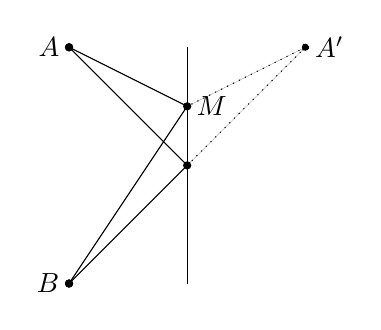
\begin{tikzpicture}[scale=1.5]
    \draw (0,2) node[left] (A) {$A$};
    \draw (2,2) node[right] (Ap) {$A'$};
    \draw (0,0) node[left] (B) {$B$};
    \draw (1,1.5) node[right] (M1) {$M$};
    \draw (1,1) node[right] (M) {};
    
    \draw (1,0) -- (1,2);
    \draw[fill=black] (A.east) circle (0.03) -- (M1.west) circle (0.03) -- (B.east) circle (0.03);
    \draw[fill=black] (A.east) circle (0.03) -- (M.west) circle (0.03) -- (B.east) circle (0.03); 
 
    \draw[dotted,fill=black] (Ap.west) circle (0.03) -- (M.west) (Ap.west) -- (M1.west);   
  \end{tikzpicture}
\end{center}
\end{minipage}%
\begin{minipage}{0.6\linewidth}
  Le chemin le plus rapide est aussi le plus court, c'est celui pour lequel les points $A'$, $M$ et $B$ sont alignés (car $AM=A'M$). On en déduit la première loi de Descartes.
\end{minipage}

\subsection{Réfraction}
\begin{center}
  \begin{tikzpicture}    
    
    %tikz optique
    \draw (0,0) -- (4,0) node[above] {$n_1$} node[below] {$n_2>n_1$};
    \draw[rayon] (0,2) -- (2,0); 
    \draw[rayon,dashed] (2,0) -- (4,2);
    \draw[rayon] (2,0) -- (3,-2);
    
    \draw[dotted] (2,-2) -- (2,2);

    \draw ([shift=(135:0.5)]2,0) arc (135:90:0.5) node[above] at ([shift=(112:0.5)]2,0) {$i_1$};

    \draw ([shift=(90:0.7)]2,0) arc (90:45:0.7) node[above] at ([shift=(67:0.7)]2,0) {$r$};

    \draw ([shift=(-90:0.5)]2,0) arc (-90:-60:0.5) node[below right] at ([shift=(-95:0.5)]2,0) {$i_2$};

  \end{tikzpicture}
  \captionof{figure}{Réfraction d'un rayon lumineux sur un dioptre entre un milieu d'indice $n_1$ et un milieu d'indice $n_2$. $i_1$ est l'angle d'incidence, $i_2$ est l'angle de réfraction et $r$ l'angle de réflexion.}
  \end{center}
  \`A l'interface entre deux milieux d'indices différents, un rayon lumineux est dévié et une partie de la lumière est réfléchie.
\begin{loi}{Seconde loi de Descartes}
\begin{itemize}
\item Le rayon réfracté appartient au plan d'incidence ;
\item $n_1\sin i_1 = n_2 \sin i_2$.
\end{itemize}
\end{loi}

\textbf{Remarques :}
\begin{itemize}
\item Si $n_2>n_1$ : Le rayon réfracté se rapproche de la normale. Il existe un angle de réfraction maximum lorsque $i_1=\pi/2$ : $i_{2_{\text{max}}} = \arcsin \left(\frac{n_1}{n_2}\right)$.
\item Si $n_2<n_1$ : Le rayon réfracté s'éloigne de la normale. Lorsque $i_2=\pi/2$, $i_{1_l}=\arcsin(\frac{n_2}{n_1})$. Si $i_1>i_{1_l}$ il y a \textbf{réflexion totale} sur l'interface qui se comporte comme un miroir.
\end{itemize}

\section{Systèmes optiques}
\subsection{Définitions}
\begin{description}
\item[Système optique :] Ensemble de milieux transparents homogènes, isotropes séparés par des surface réfringentes ou réfléchissantes.
\item[Objet :] Source (primaire ou secondaire) qui envoie des rayons lumineux vers le système optique.
\item[Image :] Point d'intersection des rayons issus du système optique et provenant d'un objet.
\item[Réel ou virtuel :] Un objet (une image) est réel(le) si les rayons qui entrent (sortent) du système optique passent effectivement par lui (elle). S'il faut prolonger les rayons pour trouver leur intersection, l'objet (l'image) est virtuel(le).
 

\textbf{Exemples :}  
\begin{itemize}
\item Systèmes optiques en transmission (dioptriques):
\begin{center}
  \begin{tikzpicture}
    %tikz optique
    \begin{scope}[shift={(0,0)}]
      \draw[fill=black] (0,0) circle (0.03) node (A1) {};
      \draw (A1.west) node[left,align=right] {$A_1$};
      \foreach \angle in {-20,-10,0,10,20}{
        \draw[rayon] (A1.center) --+ (\angle:2.5);
      }
      \draw[fill=black] (5,0) circle (0.03) node (Ap1) {};
      \draw (Ap1.east) node[right,align=left] {$A'_1$};
      \foreach \angle in {-20,-10,0,10,20}{
        \draw[rayon] (Ap1.center) ++ (\angle:-2.5) -- (Ap1.center);
      }
      \draw[draw=none,fill=white] (2,-1) to[bend left] (2,1) -- (3,1) to[bend left] (3,-1) ;
      \draw (2,-1) to[bend left] (2,1) (3,1) to[bend left] (3,-1) ;
      \draw (2.5,0) node[align=center]{Système\\ optique};
      \draw (0,-0.5) node[align=left,anchor=north]{objet réel};
      \draw (5,-0.5) node[align=left,anchor=north]{image réelle};
    \end{scope}

    \begin{scope}[shift={(9,0)}]
      \draw[fill=black] (5,0) circle (0.03) node (A1) {};
      \draw (A1.east) node[right] {$A_1$};
      \foreach \angle in {-10,-5,5,10}{
        \draw[rayon] (A1.center) ++ (\angle:-5) --++ (\angle:3);
        \draw[rayon,dotted] (A1.center) ++ (\angle:-2.5) --++ (\angle:2.5);
      }
      \draw[fill=black] (0,0) circle (0.03) node (Ap1) {};
      \draw (Ap1.west) node[left] {$A'_1$};
      \foreach \angle in {-10,-5,5,10}{
        \draw[rayon] (Ap1.center) ++ (\angle:3) --++ (\angle:2);
        \draw[rayon,dotted] (Ap1.center) --++ (\angle:2.5);
        
      }
      \draw[draw=none,fill=white] (2,-1) to[bend left] (2,1) -- (3,1) to[bend left] (3,-1) ;
      \draw (2,-1) to[bend left] (2,1) (3,1) to[bend left] (3,-1) ;
      \draw (2.5,0) node[align=center]{Système\\ optique};
      \draw (5,-1) node[align=left,anchor=north]{objet virtuel};
      \draw (0,-1) node[align=left,anchor=north]{image virtuelle};
    \end{scope}
  \end{tikzpicture}
\end{center}

\item Systèmes optiques en réflexion (catoptriques) :
\begin{center}
  \begin{tikzpicture}
    %tikz optique
    \begin{scope}[shift={(0,0)}]
      \draw[fill=black] (0,0) circle (0.03) node (A1) {};
      \draw (A1.west) node[left,align=right] {$A_1$};
      \foreach \angle in {-10,10}{
        \draw[rayon] (A1.center) --+ (\angle:3.5);
      }
      \draw[fill=black] (2,0) circle (0.03) node (Ap1) {};
      \draw (Ap1.west) node[left] {$A'_1$};
      \foreach \angle in {-30,30}{
        \draw[rayon] (Ap1.center) ++ (\angle:1) -- (Ap1.center);
      }
      \draw[draw=none,fill=white] (3,-1) to[bend left] (3,1) -- (4,1) to[bend left] (4,-1) ;
      \draw (3,-1) to[bend left] (3,1) (4,1) to[bend left] (4,-1) ;
      \draw (3.5,0) node[align=center]{Système\\ optique};
      \draw (0,0.7) node[anchor=north]{objet réel};
      \draw (1.8,-0.5) node[anchor=north]{image réelle};
    \end{scope}

    \begin{scope}[shift={(9,0)}]
      \draw[fill=black] (0,0) circle (0.03) node (A1) {};
      \draw (A1.west) node[left,align=right] {$A_1$};
      \foreach \angle in {-10,10}{
        \draw[rayon] (A1.center) --+ (\angle:2.5);
      }
      \draw[fill=black] (5,0) circle (0.03) node (Ap1) {};
      \draw (Ap1.east) node[right] {$A'_1$};
      \foreach \angle in {-6,6}{
        \draw[rayon,dotted] (Ap1.center) ++ (\angle:-2) -- (Ap1.center);
        \draw[rayon] (Ap1.center) ++ (\angle:-3) --++ (\angle:-2);
      }
      \draw[draw=none,fill=white] (2,-1) to[bend left] (2,1) -- (3,1) to[bend left] (3,-1) ;
      \draw (2,-1) to[bend left] (2,1) (3,1) to[bend left] (3,-1) ;
      \draw (2.5,0) node[align=center]{Système\\ optique};
      \draw (A1.north west) node[anchor=south east]{objet réel};
      \draw (Ap1.north) node[anchor=south]{image virtuelle};
    \end{scope}
  \end{tikzpicture}
\end{center}
\end{itemize}

\item[Axe optique :] Axe de symétrie d'un système optique
\item[Stigmatisme :] Un système est rigoureusement stigmatique si tous les rayons issus d'un point $A$ de l'objet passent par un même point $A'$ de l'image. Lorsque les rayons issus de $A$ passent tous \emph{près} de $A'$, on parle de stigmatisme approché.
\end{description}

\subsection{Le miroir plan}
\begin{center}
\begin{tikzpicture}
    %tikz optique
  \draw[very thick] (0,0) -- (7,0) ; % Miroir
  \coordinate (A) at (1,2);
  \coordinate (Ap) at (1,-2);
  \draw[fill=black] (A) circle (0.03) node[above] {$A$} ;
  \draw[fill=black] (Ap) circle (0.03) node[below] {$A'$} ;
  \draw[rayon] (A) --++ (1.5,-2);
  \draw[rayon] (A) ++ (1.5,-2) --++ (1.5,2);
  \draw[rayon,dotted] (Ap) --++ (1.5,2);
  
  \draw[rayon] (A) --++ (2.5,-2);
  \draw[rayon] (A) ++ (2.5,-2) --++ (2.5,2);
  \draw[rayon,dotted] (Ap) --++ (2.5,2);
 
  \draw[dashed] (A) -- (Ap);
  \draw (A) ++ (0,-2) --++ (0.2,0) --++ (0,0.2) --++ (-0.2,0); %angle droit
   
\end{tikzpicture}
\captionof{figure}{Construction de l'image d'un point par un miroir plan.}
\end{center}
Tous les rayons issus de $A$ passent par un même point $A'$, le système est rigoureusement stigmatique. $A$ est un objet réel et $A'$ est son image virtuelle.



\subsection{Le dioptre plan}
\begin{center}
\begin{tikzpicture}
    %tikz optique
  \draw (0,2) node[anchor=east] {$n_1$} node[anchor=west] {$n_2$} -- (0,-1); %Interface
  \coordinate (Ap) at (-5,0);
  \coordinate (A) at (-3,0); 
  \coordinate (I) at (0,1);
  \coordinate (H) at (0,0);
  \draw[fill=black] (A) node[above] {$A$} circle (0.05);
  \draw[fill=black] (Ap) node[above] {$A'$} circle (0.05); 
  \draw[rayon] (A) -- (I) ;
  \draw (I) node[below right] {$I$};
  \draw[rayon] (A) -- (H) ;
  \draw (H) node[below right] {$H$};
  \draw[rayon] (I) --++ (2,0.5);
  \draw[rayon] (H) --++(2,0);
  \draw[rayon,dotted] (Ap) -- (I);
  \draw[rayon,dotted] (Ap) -- (A);
  \draw[dashed] (I) ++ (-3,0) --++ (6,0);
  \draw ([shift=(180:1.5)]I) arc (180:198:1.5) node[left,fill=white] at ([shift=(190:1.7)]I) {$i_1$};
  \draw ([shift=(0:1.5)]I) arc (0:13:1.5) node[right,fill=white] at ([shift=(5:1.7)]I) {$i_2$};
\end{tikzpicture}
\captionof{figure}{Construction de l'image $A'$ (virtuelle) d'un point $A$ (réel) par un dioptre plan.}
\end{center}
%
On a
\begin{equation}
  \tan(i_1) = \dfrac{HI}{HA} \quad \text{et} \quad \tan(i_2)=\dfrac{HI}{HA'}
\end{equation}
%
donc 
\begin{equation}
  \dfrac{\tan(i_1)}{\tan(i_2)}=\dfrac{HA'}{HA}=\underbrace{\dfrac{\sin(i_1)}{\sin(i_2)}}_{=n_2/n_1}\dfrac{\cos(i_2)}{\cos(i_1)} \quad \text{soit} \quad \dfrac{HA'}{HA}=\dfrac{n_2}{n_1}\dfrac{\cos(i_2)}{\cos(i_1)}
\end{equation}
%
Or 
\begin{equation}
  \cos(i_2) = \sqrt{1-\sin^2(i_2)}=\sqrt{1-\left( \frac{n_1}{n_2} \right)^2\sin^2(i_1)}
\end{equation}

Donc $\dfrac{HA'}{HA} = f(i_1)$, la position de $A'$ dépend de $i_1$ il n'y a donc pas stigmatisme rigoureux.

\subsection{Stigmatisme approché, conditions de Gauss}
Pour des rayons peu inclinés par rapport à l'axe optique et proche de celui-ci (rayons \textbf{paraxiaux}) on a toujours stigmatisme approché. Ce sont les \textbf{conditions de Gauss}.

Dans le cas du dioptre plan : $i_1\ll 1$ et $i_2\ll 1$ donc $\tan(i_1)\simeq i_1$ et $\tan(i_2)\simeq i_2$ et donc
\begin{eqencadre}
  \dfrac{HA'}{HA}=\dfrac{n_2}{n_1}=\text{constante}
\end{eqencadre}
 on a donc bien stigmatisme approché.

\subsubsection{Critère de stigmatisme approché}

Généralement un système optique sert à former l'image d'un objet sur un détecteur (capteur CCD, rétine, ...) qui possède une certaine résolution (taille d'un pixel)

\begin{center}
\begin{tikzpicture}
    \begin{scope}[shift={(0,0)}]
      \draw[fill=black] (0,0) circle (0.03) node (A1) {};
      \draw (A1.west) node[left,align=right] {$A_1$};
      \foreach \angle in {-20,-10,0,10,20}{
        \draw[rayon] (A1.center) --+ (\angle:2.5);
      }
      \draw[fill=black] (5,0) node (Ap1) {};
      \draw (Ap1.east) node[right,align=left] {$A'_1$};
      \foreach \angle in {-20,-10,0,10,20}{
        \draw[rayon] (Ap1.center) ++ (\angle:-2.5) -- ($(Ap1.center) + (0,-\angle /200)$);
      }
      \draw[draw=none,fill=white] (2,-1) to[bend left] (2,1) -- (3,1) to[bend left] (3,-1) ;
      \draw (2,-1) to[bend left] (2,1) (3,1) to[bend left] (3,-1) ;
      \draw (2.5,0) node[align=center]{Système\\ optique};
      \draw (0,-0.5) node[align=left,anchor=north]{Point de l'objet};

      \draw (Ap1.center) ++ (0,-1) --++ (0,2);
      %Pixels
      \foreach \h in {-0.9,-0.7,...,0.9}{
        \draw (Ap1.center) ++ (-0.1,\h) --++ (0.2,0);
      }
 
      \draw (Ap1.center) ++ (1,1) node[right]{pixels} -- ($(Ap1.center)+ (0,0.2)$);
      \draw ($(Ap1.center) + (0,-1)$) node[below]{Détecteur}; 
    \end{scope}
\end{tikzpicture}
\end{center}
L'image $A'$ de $A$ peut être aussi étendue que la taille d'un \emph{pixel} du détecteur. La condition de stigmatisme approché est fixée par la résolution du détecteur.

\section{Lentilles sphériques minces}

\subsection{Définition}
Une lentille sphérique est un milieu transparent, homogène, isotrope limité par deux dioptres, l'un sphérique et le second plan ou sphérique. On dit que la lentille est \emph{mince} si son épaisseur est faible par rapport au rayon de courbure des faces.
\subsubsection{exemples :}
\begin{center}
\begin{tikzpicture}
\begin{scope}[shift={(0,0)}]
  \draw (0,1) to[bend right] (0,-1) to[bend right] (0,1);
  \draw (0,-1) node[below,align=center] (C1) {Lentille\\ biconvexe};
\end{scope}
\begin{scope}[shift={(2,0)}]
  \draw (0,1) to[bend right] (0,-1) to (0,1);
  \draw (0,-1) node[below,align=center] (C2) {Lentille\\ plan-convexe};
\end{scope}
\draw[decorate,decoration={brace,amplitude=10pt,mirror,raise=4pt}] (C1.south west) -- (C1.south east-|C2.south east) node[midway,yshift=-0.8cm] (LC) {Lentilles convergentes};

\draw[<->] (LC.south) -- ($(LC.south)+(0,-1)$);

\begin{scope}[shift={(5,0)}]
  \draw (0,1) to[bend left=20] (0,-1) to (0.5,-1) to[bend left=20] (0.5,1) to (0,1);
  \draw (0.25,-1) node[below,align=center] (D1) {Lentille\\ biconcave};
\end{scope}
\begin{scope}[shift={(7,0)}]
  \draw (0,1) to[bend left=20] (0,-1) to (0.5,-1) to (0.5,1) to (0,1);
  \draw (0.25,-1) node[below,align=center] (D2) {Lentille\\ plan-concave};
\end{scope}
\draw[decorate,decoration={brace, amplitude=10pt,mirror,raise=4pt}] (D1.south west) -- (D1.south east-|D2.south east) node[midway,yshift=-0.8cm] (LD) {Lentilles divergentes};
\draw[>-<] (LD.south) -- ($(LD.south)+(0,-1)$);

\draw (0,-3.5cm) node[left] {Symbole :};
\end{tikzpicture}
\captionof{figure}{Différents types de lentilles et leurs symboles.}
\end{center}

\subsection{Propriétés des lentilles minces}
\begin{itemize}
\item Les rayons passant par le \textbf{centre optique} $O$ de la lentille ne sont pas déviés.
\begin{minipage}[c]{3cm}
    \flushright
    \begin{tikzpicture}
      \draw[<->] (0,1) -- (0,-1) ;
      \draw (-1,0) -- (1,0) (0,0) node[below right,xshift=-0.1cm] {O};
      \draw[rayon,coul1] (-1,0.5) -- (0,0);
      \draw[rayon,coul1] (0,0) -- (1,-0.5); 
      \draw[rayon,coul1] (-1,-0.5) -- (0,0);
      \draw[rayon,coul1] (0,0) -- (1,0.5);
    \end{tikzpicture}
\end{minipage}

\item Les rayons parallèles à l'axe optique sortent de la lentille en passant par un même point $F'$ appelé \textbf{foyer principal image}.
\begin{center}
\begin{tikzpicture}[scale=0.5]
    %tikz optique
\begin{scope}[shift={(0,0)}]
\draw (-4,0) -- (4,0);
\draw[<->] (0,-2) -- (0,2) ;

\foreach \h in {-1.5,-0.5,0.5,1.5}{
  \draw[rayon,coul1] (-4,\h) -- (0,\h);
  \draw[rayon,coul1] (0,\h) -- (2,0) ;
  \draw[rayon,coul1] (2,0) -- (4,-\h);
}
\draw[fill=black] (2,0) circle (0.05) node[below]{$F'$} ; 
\end{scope}
\begin{scope}[shift={(12,0)}]
\draw (-4,0) -- (4,0);
\draw[>-<] (0,-2) -- (0,2) ;

\foreach \h in {-1.5,-0.5,0.5,1.5}{
  \draw[rayon,coul1] (-4,\h)  -- (0,\h);
  \draw[dotted,coul1] (-2,0) -- (0,\h) ;
  \draw[rayon,coul1] (0,\h) -- ($(4,2*\h)$);
}
\draw[fill=black] (-2,0) circle (0.05) node[fill=white,fill opacity=0.5,text opacity=1,below left]{$F'$};
\end{scope}
\end{tikzpicture}
\end{center}

\item Inversement, tous les rayons passant par le \textbf{foyer principal objet} $F$ ressortent parallèlement à l'axe optique.

\begin{center}
\begin{tikzpicture}[scale=0.5]
    %tikz optique
\begin{scope}[shift={(0,0)}]
\draw (-4,0) -- (4,0);
\draw[<->] (0,-2) -- (0,2) ;

\foreach \h in {-1.5,-0.5,0.5,1.5}{
  \draw[rayon,coul1] (-4,\h) -- (-2,0);
  \draw[rayon,coul1] (-2,0) -- (0,\h) ;
  \draw[rayon,coul1] (0,\h) -- (4,\h);
}
\draw[fill=black] (-2,0) circle (0.05) node[below]{$F$} ; 

\end{scope}
\begin{scope}[shift={(12,0)}]
\draw (-4,0) -- (4,0);
\draw[>-<] (0,-2) -- (0,2) ;

\foreach \h in {-0.9,-0.3,0.3,0.9}{
  \draw[rayon,coul1] (0,\h)  -- (4,\h);
  \draw[dotted,coul1] (0,\h) -- (2,0) ;
  \draw[rayon,coul1] ($(-4,3*\h)$)--(0,\h);
}
\draw[fill=black] (2,0) node[fill=white,fill opacity=0.5,text opacity=1,below right]{$F'$} circle (0.05) ;
\end{scope}
\end{tikzpicture}
\end{center}

\item Le plan $P$ ($P'$) perpendiculaire à l'axe optique et passant par $F$ ($F'$) est le \textbf{plan focal objet (image)}.

\item Un point de $P$ ($P'$) est un \textbf{foyer secondaire objet (image)} ;

\item La longueur algébrique $f=\ol{OF}$ est la \textbf{distance focale objet} ;
\item La longueur algébrique $f'=\ol{OF'}$ est la \textbf{distance focale image} ; $f'=-f$

\item La \textbf{vergence} $C$ d'une lentille est $C=\dfrac{1}{f'}$, on la mesure en \textbf{dioptries} ($\delta \Leftrightarrow \si{m^{-1}}$)

Pour une lentille convergente, $f'>0$ donc $C>0$. Pour une lentille divergente, $f'<0$ donc $C<0$. 
\end{itemize}

\subsubsection{remarques :}
\begin{itemize}
\item Une lentille mince est approximativement stigmatique dans les conditions de Gauss.
\item Tous les rayons qui passent pas un foyer secondaire objet ressortent parallèles entre eux.
\item Un faisseau de rayons parallèles resortent en passant par un foyer secondaire image.
  \begin{center}
    \begin{tikzpicture}[scale=0.5]
      \begin{scope}[shift={(0,0)}]
        \draw (-4,0) -- (4,0); \draw[<->] (0,-2) -- (0,2) ;

        \foreach \h in {-1.5,0,1.5}{ 
          \draw[rayon,coul1] ($(-4,0.5)+(0,\h)$) -- (0,\h); 
          \draw[rayon,coul1] (0,\h) -- ($(2,-0.5)$);
          \draw[rayon,coul1] (2,-0.5) -- ($(3,-3*0.5/2-\h/2)$);
        }
        \draw[fill=black] (2,0) circle (0.05) node[above]{$F'$};
        \draw[dotted] (2,-2) -- (2,2) node[above right] {$P'$};
      \end{scope}
      \begin{scope}[shift={(10,0)}]
        \draw (-4,0) -- (4,0); \draw[<->] (0,-2) -- (0,2) ;

        \foreach \h in {-1.5,0,1.5}{ 
          \draw[rayon,coul1] (-2,1.5) -- (0,\h); 
          \draw[rayon,coul1] (0,\h) -- ($(3,\h-2.25)$);
          %\draw[rayon,coul1] (2,-0.5) -- ($(3,-3*0.5/2-\h/2)$);
        }
        \draw[fill=black] (-2,0) circle (0.05) node[above]{$F$};
        \draw[fill=black] (2,0) circle (0.05) node[above]{$F'$};
        \draw[dotted] (-2,-2) -- (-2,2) node[above right] {$P$};
      \end{scope}
    \end{tikzpicture}
  \end{center}
\end{itemize}

\subsection{construction des images}
\subsubsection{Objet à distance finie}
\begin{center}
\begin{tikzpicture}
    %tikz optique
\begin{scope}[shift={(0,0)}]
\def\Fp{1.5}
\def\OA{-4}
\def\AB{1.5}
\pgfmathsetmacro{\OAp}{(\OA*\Fp/(\OA+\Fp)}
\pgfmathsetmacro{\ApBp}{\AB*\OAp/\OA}

\draw (-4,0) -- (4,0); \draw[<->] (0,-2) -- (0,2) ; % axe, lentille
\draw[->] (\OA,0) node[below] {$A$} -- (\OA,\AB) node[above] {$B$} coordinate (B); %objet
\draw[->] (\OAp,0) node[above] {$A'$} --++ (0,\ApBp) node[below] {$B'$} coordinate (Bp); %image

\draw[fill=black] (-\Fp,0) circle (0.05) node[below] {$F$} coordinate (F);
\draw[fill=black] (\Fp,0) circle (0.05) node[above] {$F'$} coordinate (Fp);

\draw[rayon, coul1] (B) -- ($(B)+(4,0)$) coordinate (C) ;
\draw[rayon, coul1] (C) -- (Fp) ;
\draw[rayon, coul1] (Fp) -- (Bp) ;

\draw[rayon] (B) -- (0,0);
\draw[rayon] (0,0) -- (Bp);

\draw[rayon] (B) -- (0,\ApBp);
\draw[rayon] (0,\ApBp) -- (\OAp,\ApBp);

\draw (\OA,-0.5) node[below] {Objet réel};
\draw (\OAp,0.5) node[above] {Image réelle};
\end{scope}

\begin{scope}[shift={(10,0)}]
\def\Fp{-2}
\def\OA{-4}
\def\AB{1.5}
\pgfmathsetmacro{\OAp}{(\OA*\Fp/(\OA+\Fp)}
\pgfmathsetmacro{\ApBp}{\AB*\OAp/\OA}

\draw (-4,0) -- (3,0); \draw[>-<] (0,-2) -- (0,2) ; % axe, lentille
\draw[->] (\OA,0) node[below] {$A$} -- (\OA,\AB) node[above] {$B$} coordinate (B); %objet
\draw[->] (\OAp,0) node[below] {$A'$} --++ (0,\ApBp) node[above] {$B'$} coordinate (Bp); %image

\draw[fill=black] (-\Fp,0) circle (0.05) node[below] {$F$} coordinate (F);
\draw[fill=black] (\Fp,0) circle (0.05) node[above] {$F'$} coordinate (Fp);

\draw[rayon, coul1] (B) -- ($(B)+(4,0)$) coordinate (C) ;
\draw[rayon, dotted] (Fp) -- (C) ;
\draw[rayon, coul1] (C) -- ($(C)+0.4*(C)-0.4*(Fp)$) ;

\draw[rayon] (B) -- (0,0);
\draw[rayon] (0,0) -- ($-0.5*(B)$);

\draw[rayon] (B) -- (0,\ApBp);
\draw[rayon] (0,\ApBp) --++ (2,0);
\draw[rayon,dotted] (0,\ApBp) -- (F);
\draw[rayon,dotted] (Bp) -- (0,\ApBp); 

\draw (\OA,-0.5) node[below] {Objet réel};
\draw (\OAp,-0.5) node[below] {Image virtuelle};
\end{scope}
\end{tikzpicture}
\end{center}

\begin{center}
\begin{tikzpicture}
\begin{scope}[shift={(0,0)}]
\def\Fp{2}
\def\OA{4}
\def\AB{1.5}
\pgfmathsetmacro{\OAp}{(\OA*\Fp/(\OA+\Fp)}
\pgfmathsetmacro{\ApBp}{\AB*\OAp/\OA}

\draw (-4,0) -- (4,0); \draw[<->] (0,-2) -- (0,2) ; % axe, lentille
\draw[->] (\OA,0) node[below] {$A$} -- (\OA,\AB) node[above] {$B$} coordinate (B); %objet
\draw[->] (\OAp,0) node[below] {$A'$} --++ (0,\ApBp) node[above] {$B'$} coordinate (Bp); %image

\draw[fill=black] (-\Fp,0) circle (0.05) node[below] {$F$} coordinate (F);
\draw[fill=black] (\Fp,0) circle (0.05) node[above] {$F'$} coordinate (Fp);

\draw[rayon] (-4,\AB) -- (0,\AB) coordinate (C) ;
\draw[rayon,dotted] (C) -- (B);
\draw[rayon] (C) -- (Fp) ;

\draw[rayon] ($(F)-0.3*(B)+0.3*(F)$) -- ($(F)+0.333*(B)-0.333*(F)$) coordinate (D);
\draw[rayon,dotted] (D) -- (B);
\draw[rayon] (D) -- ($(Bp)+(1,0)$);

\draw[rayon] (-\OA,-\AB) -- (0,0);
\draw[rayon] (0,0) -- (B);

\draw (\OA,-0.5) node[below] {Objet virtuel};
\draw (\OAp,-0.5) node[below] {Image réelle};
\end{scope}

\begin{scope}[shift={(10,0)}]
\def\Fp{2}
\def\OA{-2}
\def\AB{1}

\draw (-4,0) -- (3,0); \draw[<->] (0,-2) -- (0,2) ; % axe, lentille
\draw[->] (\OA,0) node[below right] {$A$} -- (\OA,\AB) node[above] {$B$} coordinate (B); 

\draw[fill=black] (-\Fp,0) circle (0.05) node[below left] {$F$} coordinate (F);
\draw[fill=black] (\Fp,0) circle (0.05) node[above] {$F'$} coordinate (Fp);

\draw[rayon, coul1] (B) -- ($(B)+(2,0)$) coordinate (C) ;
\draw[rayon, coul1] (C) -- (Fp) ;
\draw[rayon, coul1] (Fp) -- ($(Fp)+(Fp)-(C)$);

\draw[rayon] (B) -- (0,0);
\draw[rayon] (0,0) -- ($-1*(B)$); 

\draw[->] ($(Fp)+(0.3,0.3)$) --++ (0.6,0) node[midway,above] {$A'$};
\draw[->] ($0.5*(Fp)-0.2*(B)$) --++ ($-0.3*(B)$) node[at end,right,sloped] {$B'$};

\draw (\OA,-0.5) node[below] {Objet réel};
\draw (\Fp,-1) node[below right] {Image à l'infini};
\end{scope}
\end{tikzpicture}
\end{center}

\subsubsection{objet à l'infini : }
Les rayons provenant d'un point situé à l'infini sont tous parallèles entre eux 

\vspace{1em}
\noindent\begin{minipage}{0.5\linewidth}
  \begin{center}
    \begin{tikzpicture}

\def\Fp{2}
\def\ApBp{-1}

\draw (-4,0) -- (4,0); \draw[<->] (0,-2) -- (0,2) ; % axe, lentille
\draw[->] (\Fp,0) node[above right] {$A'$} --++ (0,\ApBp) node[below] {$B'$} coordinate (Bp); %image

\draw[fill=black] (-\Fp,0) circle (0.05) node[below] {$F$} coordinate (F);
\draw[fill=black] (\Fp,0) circle (0.05) node[above left] {$F'$} coordinate (Fp);

\coordinate (C) at ($(Bp) - (\Fp,0)$);
\draw[rayon] ($(C)-2*(Bp)$) -- (C) ;
\draw[rayon] (C) -- (Bp) ;
\draw[rayon] ($-2*(Bp)$) -- (Bp) ;

\draw[->] ($(-\Fp-0.5,-0.2)$) --++ (-0.7,0) node[midway, below] {$A_{\infty}$};
\draw[->] ($-0.5*(Bp)+(0,0.3)$) --++ ($-0.5*(Bp)$) node[midway,sloped,above]{$B_{\infty}$};
    \end{tikzpicture}
  \end{center}
\end{minipage}%
\begin{minipage}{0.5\linewidth}
L'image d'un objet situé à l'infini est dans le plan focal image de la lentille.
\end{minipage}

Dans tous les cas, pour construire l'image, on utilise les propriétées particulières des rayons passant par $O$,$F$ et $F'$.

\subsection{Formules de conjugaison}
On cherche une relation mathématique entre les positions de $A$ et de son image  $A'$, tous deux étant sur l'axe optique.

%\noindent\begin{minipage}{0.5\linewidth}
\begin{center}
  \begin{tikzpicture}
    \def\Fp{1.5}
\def\OA{-4}
\def\AB{1.5}
\pgfmathsetmacro{\OAp}{(\OA*\Fp/(\OA+\Fp)}
\pgfmathsetmacro{\ApBp}{\AB*\OAp/\OA}

\draw (-4,0) -- (4,0); \draw[<->] (0,-2) -- (0,2) ; % axe, lentille
\draw[->] (\OA,0) node[below] {$A$} -- (\OA,\AB) node[above] {$B$} coordinate (B); %objet
\draw[->] (\OAp,0) node[above] {$A'$} --++ (0,\ApBp) node[below] {$B'$} coordinate (Bp); %image

\draw[fill=black] (-\Fp,0) circle (0.05) node[below] {$F$} coordinate (F);
\draw[fill=black] (\Fp,0) circle (0.05) node[above] {$F'$} coordinate (Fp);

\draw[rayon, coul1] (B) -- ($(B)+(4,0)$) coordinate (C) ;
\draw (C) node[above right]{$H$}; 
\draw[rayon, coul1] (C) -- (Fp) ;
\draw[rayon, coul1] (Fp) -- (Bp) ;

\draw[rayon] (B) -- (0,0);
\draw[rayon] (0,0) -- (Bp);

\draw (0,0) node[above right] {$O$};

\draw[rayon] (B) -- (0,\ApBp) coordinate (K);
\draw (K) node[below left]{$K$}; 
\draw[rayon] (0,\ApBp) -- (\OAp,\ApBp);
  \end{tikzpicture}
  \end{center}

  On applique le théorème de Thalès : $\dfrac{\ol{AB}}{\ol{A'B'}} = \dfrac{\ol{OA}}{\ol{OA'}} = \dfrac{\ol{FA}}{\ol{FO}}$ avec $\ol{FA}=\ol{FO}+\ol{OA}$, on obtient : $\dfrac{\ol{OA}}{\ol{OA'}}=1+\dfrac{\ol{OA}}{\ol{FO}}$. D'où :

  \begin{loi}{Formule de conjugaison de Descartes}
  \begin{equation}
    \frac{1}{\ol{OA'}}-\frac{1}{\ol{OA}} = \frac{1}{f'}
  \end{equation}
  \end{loi}

En appliquant le théorème de Thalès de chaque côté de la lentille, on obtient aussi :
\begin{equation*}
  \frac{\ol{FA}}{\underbrace{\ol{FO}}_{f'}} = \frac{\ol{AB}}{\ol{A'B'}} \quad \text{et} \quad \frac{\ol{F'A'}}{\underbrace{\ol{F'O}}_{-f'}} = \frac{\ol{A'B'}}{\ol{AB}} 
\end{equation*}

\begin{loi}{Formule de conjugaison de Newton}
\begin{equation}
    \ol{FA}\cdot\ol{F'A'} = -f'^2
\end{equation}
\end{loi}

\begin{loi}{Grandissement transversal}
  Le grandissement transversal relatif à une objet $AB$ et son image $A'B'$ est défini comme
\begin{equation}
  G_t=\frac{\ol{A'B'}}{\ol{AB}}
\end{equation}
Et on a les relations
\begin{equation}
  G_t = \frac{\ol{OA'}}{\ol{OA}}  \quad \text{et}\quad G_t= \frac{f'}{\ol{FA}} = -\frac{\ol{F'A'}}{f'}
\end{equation}
\end{loi}

Considérons un objet $A$ réel dont l'image $A'$ par une lentille convergente est réelle. On note $D$ la distance $\ol{AA'}$ et $x$ la distance $\ol{AO}$. En appliquant la formule de conjugaison de Descartes, on a :
\begin{equation*}
  \frac{1}{\ol{OA'}}-\frac{1}{\ol{OA}} = \frac{1}{f'} \text{ soit } \frac{1}{D-x} + \frac{1}{x} = \frac{1}{f'}
\end{equation*}
On cherche où doit être placée la lentille pour que l'image de $A$ soit en $A'$. il faut donc déterminer $x$, l'équation précédente devient :
\begin{equation*}
  \frac{x+(D-x)}{x(D-x)} = \frac{1}{f'} \Leftrightarrow \frac{D}{x(D-x)} = \frac{1}{f'} \Leftrightarrow x^2-Dx+f'D = 0
\end{equation*}

On obtient une équation du second degré. Il existe une solution réelle à condition que $\Delta = D^2-4f'D \geq 0$ soit $D\geq 4f'$. Un objet réel possède donc une image réelle par une lentille convergente à condition que l'objet et l'image soit séparés d'au moins 
\begin{eqencadre}
  D\geq 4f'
\end{eqencadre}
C'est la distance minimale entre un objet et l'écran sur lequel on veut projeter son image par une lentille convergente. 

\section{Quelques dispositifs optiques}
\subsection{L'\oe{}il}
\begin{center}
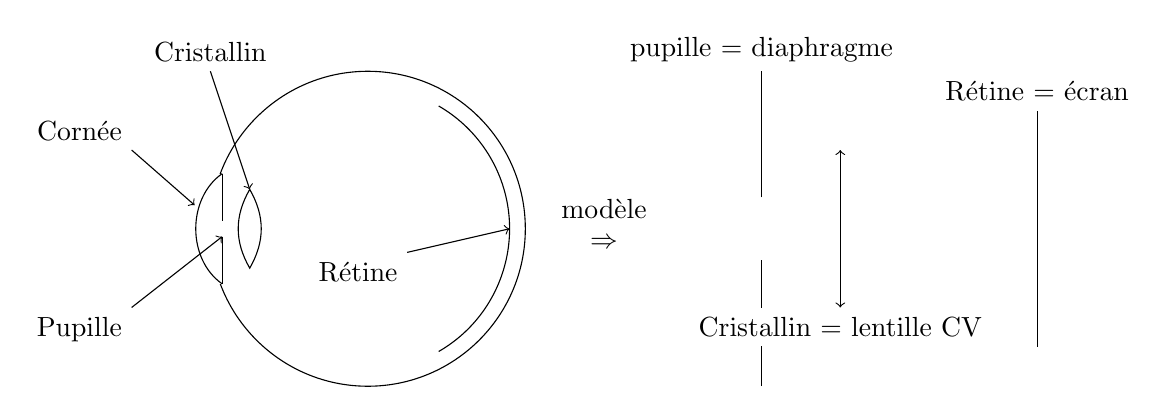
\begin{tikzpicture}
    %tikz optique
\draw (2,0) circle(2);
\draw ([shift={(-60:1.8)}]2,0) arc(-60:60:1.8);
\newcommand{\rCorn}{0.7}
\draw[fill=white,draw=none] (-0.1,-\rCorn) rectangle (2,\rCorn);

\newcommand{\xCorn}{0.15}
\draw (\xCorn,\rCorn) to[bend right=55] (\xCorn,-\rCorn) coordinate[midway] (Corn);

\newcommand{\xCris}{0.5}
\newcommand{\rCris}{0.5}
\draw (\xCris,\rCris) to[bend right]  (\xCris,-\rCris) to[bend right] (\xCris,\rCris) coordinate (Cris) ;

\draw (\xCorn,\rCorn) -- (\xCorn,0.1)  (\xCorn,-0.1) coordinate (Pup) -- (\xCorn,-\rCorn);

\draw[<-] (-0.2,0.3) -- (-1,1) node[above left] {Corn\'ee};
\draw[<-] (Pup) -- (-1,-1) node[below left] {Pupille};
\draw[<-] (Cris) -- (0,2) node[above] {Cristallin};
\draw[<-] (3.8,0) -- (2.5,-0.3) node[below left] {R\'etine};


\draw (5,0) node[below] {$\Rightarrow$} node[above]{mod\`ele};
\draw (7,-2) --  (7,-0.4) (7,0.4) -- (7,2) node[above] {pupille = diaphragme};
\draw[<->] (8,1) -- (8,-1) node[below,fill=white] {Cristallin = lentille CV};
\draw (10.5,-1.5) -- (10.5,1.5) node[above]{R\'etine = \'ecran};
\end{tikzpicture}
\captionof{figure}{Principe de fonctionnement de l'\oe{}il et modélisation.}
\end{center}
Le cristallin forme l'image des objets sur la rétine.

Le cristallin est une lentille convergente de vergence variable qui se déforme pour former l'image de l'objet observé sur la rétine. C'est l'\textbf{accomodation}. 

\begin{itemize}
\item Au repos le cristallin n'accomode pas, les objets dont l'image est nette sont au \textbf{punctum remotum} ($PR$). Pour un \oe il normal, $PR = \infty$.

\item Quand il accomode au maximum, le cristallin forme sur la rétine l'image des objets situés au \textbf{punctum proximum} ($PP$). Pour un \oe il normal, $PP\simeq\SI{25}{cm}$.
\end{itemize}

L'accomodation permet de voir nets les objets situés entre ($PP$) et ($PR$).

\begin{center}
  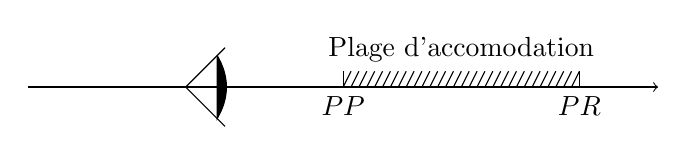
\begin{tikzpicture}
   \draw[->] (0,0) -- (8,0);
   \draw (2,0) --+(0.5,0.5) (2,0) --+(0.5,-0.5);
   \draw[fill=black] (2.4,0.4) to[bend left] (2.4,-0.4) -- (2.4,0.4);
   \draw (4,0) node[below] {$PP$} -- (4,0.2);
   \draw (7,0) node[below] {$PR$} -- (7,0.2);
   \foreach \x in {4,4.1,...,7}{
     \draw (\x,0) --++ (0.1,0.2);
   }
   \draw (5.5,0.2) node[above]{Plage d'accomodation};
  \end{tikzpicture}
  \captionof{figure}{Définition de la plage d'accommodation.}
\end{center}

Le pouvoir de résolution de l'\oe{}il détermine la taille du plus petit objet que l'on puisse discerner.

\noindent\begin{minipage}{0.5\linewidth}
\begin{center}
\begin{tikzpicture}[scale=0.7]
  \draw[->] (-5,0) -- (4,0);
  \draw[<->] (0,-2) -- (0,2);
  \draw[->] (-4,0) node[below] {$A$} -- (-4,2) coordinate (B) node[above]{$B$};
  \draw[->] (3,0) node[above] {$A'$} -- (3,-1.5) coordinate (Bp) node[below]{$B'$};
  \draw[rayon] (B) -- (Bp);
  
  \draw (0.8,0) arc(0:-28:0.8);
  \draw (0.8,0) node[below right] {$\alpha$};
  \draw[<->] (0.1,1) -- (2.9,1) node[midway,above]{$d=\SI{15}{mm}$};
\end{tikzpicture}
\end{center}
\end{minipage}%
\begin{minipage}{0.5\linewidth}
 Pour être distingués, les points $A$ et $B$ doivent être séparés d'au moins une cellule soit $\simeq \SI{5}{\micro m}$

$\alpha \approx \tan(\alpha) = \dfrac{A'B'}{d} = \dfrac{\SI{5}{\micro m}}{\SI{15e-3}{m}}\simeq \SI{3e-4}{rad}$.
\end{minipage} 

L'\oe il ne peut distinguer des objets séparés angulairement de moins de \SI{3e-4}{rad}. Cela correspond à une distance de :
\begin{itemize}
\item $\num{3e-4}\times\SI{25}{cm}=\SI{75}{\micro m}$ au ($PP$);
\item $\num{3e-4}\times\SI{400000}{km}=\SI{120}{km}$ au sur la Lune;
\end{itemize}

\subsection{L'appareil photographique}%
\label{sub:l_appareil_photographique}
On peut modéliser un appareil photographique par l'association d'une lentille convergente, d'un diaphragme et d'un capteur. L'objectif forme sur le capteur l'image de l'objet photographié.

\begin{center}
\begin{tikzpicture}[scale=1, transform shape]
    %tikz optique
\draw[-latex] (0,0) -- (12,0) node[right]{Axe optique};
\draw[<->] (5,-2) -- (5,2) node[above left, align=right]{Objectif\\distance focale image $f$};
\draw[very thick] (5.3,-2) -- (5.3, -0.5) (5.3, 0.5) -- (5.3, 2) node[above right, align=left, text width=3cm]{Diaphragme\\diametre d'ouverture $d$};
\coordinate (A) at (1,0);
\draw (9,-2) -- (9,2) node[above right] {Capteur};
\draw[rayon, gray] (A) -- (5,1) -- (5.3, 0.92);
\draw[rayon, gray] (A) -- (5,0.5);
\draw[rayon, gray] (5,0.5) -- (9,0);
\draw[rayon, gray] (A) -- (5,-0.5);
\draw[rayon, gray] (5,-0.5) -- (9,0);
\draw[rayon, gray] (A) -- (5,-1) -- (5.3,-0.92);
\draw[<->] (5.4,-2) -- (8.9, -2) node[midway, below]{$D$};
\draw[fill=black] (1,0) circle(0.5mm) node[below left, align=right, text width=3cm] {Point de l'objet dans le plan de mise au point};
\draw[fill=black] (9,0) circle(0.5mm) node[below right, text width=3cm, align=left] {Point de l'image dans le plan du capteur};
\node[above right, text width=3cm]  (n1) at (9.5,0.5){L'image sur le capteur est un point};
\draw (n1.south west) -- (9,0) ;
\end{tikzpicture}
\captionof{figure}{Principe de fonctionnement d'un appareil photographique.}
\end{center}

La distance focale de l'objectif détermine le \textit{zoom} de l'appareil (ou la largeur de champ). L'ouverture du diaphragme joue principalement sur la quantité de lumière reçue par le capteur, mais aussi sur la \textbf{profondeur de champ}, qui correspond à la zone dans laquelle peut se trouver un objet pour que son image soit nette.

\begin{center}
\begin{tikzpicture}[scale=1, transform shape]
\draw[-latex] (0,0) -- (14,0) node[right]{Axe optique};
\draw[<->] (5,-2) -- (5,2) node[above left, align=right]{Objectif};
\draw[very thick] (5.3,-2) -- (5.3, -0.8) (5.3, 0.8) -- (5.3, 2) node[above right, align=left, text width=3cm]{Diaphragme};
\draw (9,-2) -- (9,2) node[above right] {Capteur};
\foreach \y in {-2,-1.2,...,2.1}{\draw (9,\y) -- ++(0.2,0);}
\coordinate (A) at (1.5,0);
%\draw[rayon, gray!50] (A) -- (5,1) -- (5.3, 0.92);
\draw[rayon, gray!50] (A) -- (5,0.8);
\draw[rayon, gray!50] (5,0.8) -- (9,0);
\draw[rayon, gray!50] (A) -- (5,-0.8);
\draw[rayon, gray!50] (5,-0.8) -- (9,0);
%\draw[rayon, gray!50] (A) -- (5,-1) -- (5.3,-0.92);

\coordinate (B) at (0,0);
%\draw[rayon, ] (B) -- (5,1) -- (5.3, 0.87);
\draw[rayon, black ] (B) -- (5,0.8);
\draw[rayon, black ] (5,0.8) -- (9,-0.4);
\draw[rayon, black ] (B) -- (5,-0.8);
\draw[rayon, black ] (5,-0.8) -- (9,0.4);
%\draw[rayon, ] (B) -- (5,-1) -- (5.3,-0.87);


\coordinate (C) at (2.5,0);
%\draw[rayon, ] (C) -- (5,1) -- (5.3, 0.87);
\draw[rayon, gray] (C) -- (5,0.8);
\draw[rayon, gray ] (5,0.8) -- (12,0);
\draw[rayon, gray ] (C) -- (5,-0.8);
\draw[rayon, gray ] (5,-0.8) -- (12,0);
%\draw[rayon, ] (C) -- (5,-1) -- (5.3,-0.87);

\draw[fill=black] (C) circle(0.5mm);
\draw[fill=black] (B) circle(0.5mm);
\draw[dotted] (C) -- ++(0, -1);
\draw[dotted] (B) -- ++(0, -1);
\draw[<->] ($(C)+(0,-1)$) -- ($(B)+(0,-1)$) node[midway, below]{Profondeur de champ};

\draw[latex-] (9.2, 1.6) -- ++(1,0) node[right]{pixel};
\end{tikzpicture}
\captionof{figure}{Construction géométrique de la profondeur de champ d'un appareil photographique pour un réglage donné.}
\end{center}

\subsection{La fibre optique à saut d'indice}%
\label{sub:la_fibre_optique_a_saut_d_indice}
Une fibre optique permet de guider la lumière en lui faisant subir une succession de réflexions totales à l'intérieur d'un milieu d'indice $n_1$ entouré d'un milieu d'indice $n_2<n_1$. 

\begin{center}
  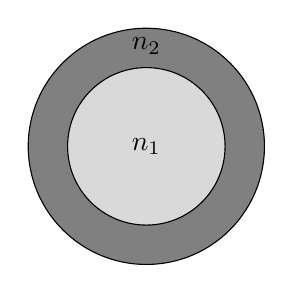
\begin{tikzpicture}
    \draw[fill=gray] (0,0) circle (1.5cm) ;
    \draw[fill=gray!30] (0,0) circle (1cm);
    \draw (0, 1.5) node[below]{$n_2$}; 
    \draw (0, 0) node[]{$n_1$}; 
  \end{tikzpicture}
  \captionof{figure}{Coupe transversale d'une fibre optique à saut d'indice.}
\end{center}

\begin{center}
  \begin{tikzpicture}
    %tikz optique
    \fill[gray](0, -1.5) rectangle (10, 1.5);
    \fill[gray!30](0, -1) rectangle (10, 1);
    \foreach \y in {1.5, 1, -1, -1.5} {
      \draw[] (0, \y) -- (10, \y);    
    }
  \draw[dashed] (-1.5, 0) -- (10,0);
  \draw[rayon,black] (0,0) ++ (220: 2) -- (0,0); 
  \draw[rayon,black] (0,0)  -- ++({1/tan(30)},1) coordinate (B); 
  \draw[rayon,black] (B)  -- ++({2/tan(30)},-2) coordinate (C); 
  \draw[rayon,black] (C)  -- ++({2/tan(30)},2) coordinate (C); 
  \draw (-0.5, 0) arc(180:220:0.5) node[midway, left, yshift=-4px] {$i_0$};
  \draw (0.5, 0) arc(0:30:0.5) node[midway, right, yshift=2px] {$i$};
  \draw (B) node[above left]{$B$};
  \draw (0,0) node[above left]{$A$};
  \draw[dashed] (B) ++ (0, 0.5) -- ++(0, -1.3);
  \draw (B) ++ (0, -0.5) arc(-90:-150:0.5) node[midway, below left] {$i_1$ };
  \draw (B) ++ (0, -0.5) arc(-90:-30:0.5) node[midway, below right] {$i_1$ };
  \draw (5,1) node[below]{$n_1$} node[above]{$n_2<n_1$ };  
  \end{tikzpicture}
\captionof{figure}{Coupe longitudinale d'une fibre optique à saut d'indice et rayon lumineux limite confiné à l'intérieur de la fibre.}
\end{center}

Pour une fibre optique à saut d'indice, le \textbf{cône d'acceptance} correspond au cône dans lequel doit se trouver un rayon lumineux incident pour subir des réflexions totales à l'intérieur de la fibre. 

Il s'agit de déterminer l'angle d'incidence $i_0$ limite pour lequel un rayon lumineux subit une réflexion totale en $B$.

Les lois de la réfraction en $A$ donnent 
\begin{equation}
  \sin(i_0) = n_1\sin(i) = n_1\cos(i_1)
\end{equation}

Or l'angle $i_1$ limite pour lequel il y a réflexion totale est donné par
\begin{equation}
  n_1 \sin(i_1) = n_2 = n_1 \sqrt{1-\cos^2(i_1)} \quad \text{donc} \quad \cos(i_1) = \sqrt{1-\frac{n_2^2}{n_1^2}}
\end{equation}
et finalement
\begin{eqencadre}
  \sin(i_0) = \sqrt{n_1^2 - n_2^2}
\end{eqencadre}
Les rayon arrivant avec une incidence plus importante se seront pas guidés dans la fibre.

On voit alors que si l'on envoie sur la fibre deux rayons lumineux, l'un arrivant en incidence normale et l'autre avec l'incidence maximale, les temps de parcours des deux rayons dans une fibre de longueur $L$  seront différents.

La différence de temps par unité de longueur entre le temps de parcours le plus long et le temps de parcours le plus faible dans la fibre est appelée \textbf{dispersion intermodale} et notée $\Delta t_\text{im}$ (en \si{\second\per\meter}). On peut montrer que 
\begin{equation}
  \Delta t_\text{im} = \frac{t(i_0)-t(0)}{L}= \frac{\frac{Ln_1}{c\cos(i)}-\frac{Ln_1}{c}}{L} = \frac{n_1}{c\cos(i)}-\frac{n_1}{c} = \frac{n_1}{c}\left( \frac{1}{\cos(i)}-1 \right) 
\end{equation}
Or on a 
\begin{equation}
  \cos(i) = \sqrt{1-\sin^2(i)} = \sqrt{1-\frac{\sin^2(i_0)}{n_1^2}} = \sqrt{1-\frac{n_1^2-n_2^2}{n_1^2}} = \frac{n_2}{n_1}
\end{equation}
et donc on obtient
\begin{eqencadre}
  \Delta t_\text{im}=\frac{n_1}{c}\frac{n_1-n_2}{n_2}
\end{eqencadre}
La dispersion intermodale limite le débit maximum des données qui peuvent circuler dans la fibre.
\end{document}
%%% Local Variables: 
%%% mode: latex
%%% LaTeX-command: "latex -shell-escape"
%%% End: 
